\chapter{FTSP+} \label{cap:cap4}
\outlineon=0

\outline{
  \begin{itemize}
    \item Explicar a t�cnica.
    \item Inserir ilustra��o do processo de sincroniza��o com o rel�gio externo. 
    \item Pseudo c�digo
    \item FTSP+ e subsection
  \end{itemize}
}

As principais t�cnicas para o c�lculo e estimativa do atraso trabalham com \textit{timestamp} no n�vel de acesso ao meio ou com a troca de mensagens, ambas s�o custosas, visto que mecanismos de marca��o de tempo na camada MAC s�o dependentes de \textit{hardware} espec�fico e a troca de mensagens quebra com a premissa unidirecional do FTSP. N�s propusemos ent�o o FTSP+ que substitui o recurso de MAC \textit{timestamp} por um \textit{timestamp} a n�vel de aplica��o, baseado na ideia de que um n� � capaz de determinar no envio de uma mensagem quando ela termina de ser enviada, ent�o � poss�vel calcular os atrasos no processo de envio e com uma mensagem posterior efetuar a corre��o do \textit{timestamp}. Esta m�todo j� foi previamente discutido por \cite{sousa2014stele} que � uma t�cnica simples de estimativa de atraso local para RSSF.


\section{T�cnica}

\outline{Descrever o processo de c�lculo do tempo de acesso ao meio, e onde foi baseado.}


Em qualquer t�cnica de sincroniza��o de rel�gios em sistemas distribu�dos, os n�s tem que dizer um ao outro o seu tempo local. A Figura \ref{fig:diagrama} ilustra esse cen�rio. O n� emissor armazena o seu tempo local ${t_1}'$ na mensagem de sincroniza��o no tempo $t_1$ e ordena o envio da mensagem. Devido as incertezas aleat�rias do acesso ao meio, o emissor s� recebe o acesso ao meio no tempo $t_2$ e come�a a enviar a mensagem. O \textit{tempo de acesso ao meio} � definido por $t_2 - t_1$. A mensagem propaga-se sobre o meio por um intervalo de tempo $tp$ at� que atinge o r�dio do receptor no tempo $t_3$. O \textit{tempo de propaga��o} � definido por $tp$. Devido as pol�ticas de manipula��o de interrup��o e processamento do cabe�alho do pacote, o n� receptor marca o \textit{timestamp} do recebimento no tempo $t_4$ com o seu tempo local ${t_4}''$. O \textit{tempo de processamento} � dado por $t_4 - t_3$.



\begin{figure}[htbp]
	\centering
		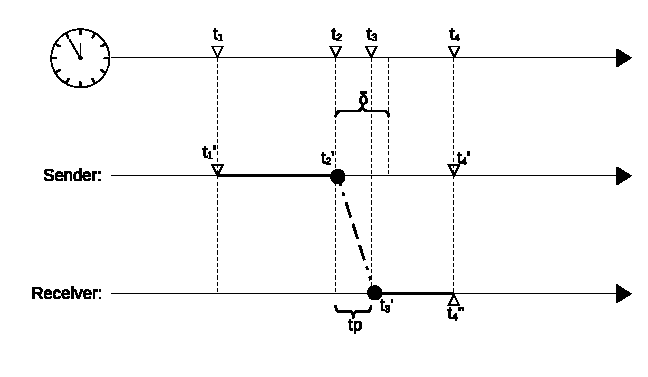
\includegraphics[width=\linewidth]{figuras/diagrama.eps}
	\caption{Syncronization steps.}
	\label{fig:diagrama}
\end{figure}


A imprecis�o de sincroniza��o acontece porque o n� de receptor pensa que no tempo $t_4$ o emissor tem o tempo ${t_1}'$ e o receptor tem o tempo ${t_4}''$. Como podemos ver na Figura \ref{fig:diagrama}, isso n�o � verdade. No tempo $t_4$, o n� emissor tem o tempo ${t_4}' = {t_1}' + \mbox{\textit{tempo de acesso ao meio}} + \mbox{\textit{tempo de propaga��o}} + \mbox{\textit{tempo processamento}}$. O \textit{timestamp} na camada MAC faz \textit{tempo de acesso ao meio} e \textit{tempo de processamento} igual a zero. Desde que o \textit{tempo de propaga��o} � desprez�vel ($\sim 1\mu{s}$) \cite{maroti2004}, algumas pol�ticas de sincroniza��o -- incluindo o FTSP -- podem atingir uma precis�o muito boa. Contudo, sem o \textit{timestamp} na camada MAC, esses tempo n�o s�o negligenci�veis e tem que ser calculados. 


\section{Modifica��o}\label{sec:mod}

\outline{
   Pseudo c�digo com explica��o do passo-a-passo do algoritmo (no sender e no receiver).
}


O FTSP+ calcula o \textit{tempo de acesso ao meio} usando uma manipula��o de interrup��o para marcar o tempo do momento que o n� obt�m o acesso ao meio para enviar a mensagem de sincroniza��o. Embora o acesso ao meio � concedido no tempo ${t_2}'$, \textit{timestamp de acesso ao meio} � igual a ${t_2}'+\delta$, onde $\delta$ � o \textit{overhead} para processar a manipula��o da interrup��o.



O emissor envia uma mensagem com o conte�do ${t_2}'+\delta-{t_1}'$ ent�o o receptor pode estimar ${t_4}'$. Vamos chamar esta estimativa de $\bar{{t_4}'}$. O receptor calcula $\bar{{t_4}'}$ as in Equa��o \eqref{eq:estimated_t4}.



\begin{eqnarray}
\bar{t4'} & = & t1' - (t2' + \delta - t1') \nonumber\\
\label{eq:estimated_t4}
\bar{t4'} & = & t1' + \mbox{\textit{tempo de acesso ao meio}} + \delta
\end{eqnarray}



A estimativa de erro � a diferen�a entre ${t_4}'$ e $\bar{t_4}'$, que �:
\begin{equation}
\label{eq:estimation_error}
t4' - \bar{t4'} = \mbox{\textit{tempo de propaga��o}} + \mbox{\textit{tempo de processamento}} - \delta
\end{equation}

Desde de que o \textit{tempo de processamento} e o $\delta$ s�o lat�ncias do processamento da manipula��o de interrup��o. 
N�s investigamos seus valores em nosso experimento no Cap�tulo \ref{cap:cap5}, eles tendem a anular-se mutuamente. Relembrando que o \textit{tempo de propaga��o} � negligenci�vel.




\begin{figure}
\begin{Verbatim}[numbers=left,numbersep=1pt,frame=single]
event Radio.receiveSyncMsg(SyncMsg *msg){
  if( msg->rootID < myRootID )
      myRootID = msg->rootID;
  else if( msg->rootID > myRootID
    || msg->seqNum <= highestSeqNum )
      return;
  highestSeqNum = msg->seqNum;
  if( myRootID < myID )
      heartBeats = 0;
  if( numEntries >= NUMENTRIES_LIMIT
    && getError(msg) > TIME_ERROR_LIMIT )
      clearRegressionTable();
  else if (MAC_Time==false){
      addToWaitCorrectionMsgList(msg);
  }else{
      addEntryAndEstimateDrift(msg); 
  }  
}

event Radio.receiveCorrectionMsg(
                            CorrectionMsg *msg){
  applyCorrection(msg);
  addEntryAndEstimateDrift(msg);
}
\end{Verbatim}
 \caption{Algoritmo do receptor.}\vspace{1em}
 \label{fig:receiver_ftspplus}
\end{figure}

Como podemos ver na Figura \ref{fig:receiver_ftspplus}, o receptor FTSP+ tem rotinas para manipular dois tipos diferentes de mensagens de recebimento: \texttt{Radio.receiveSyncMsg(SyncMsg *msg)} serve para as mensagens de sincroniza��o e o \texttt{Radio.receiveCorrectionMsg(CorrectionMsg *msg)} � utilizado nas mensagens de corre��o. O \textit{tempo de corre��o}, expressado na Equa��o (\ref{eq:correction_time}), � a informa��o que � transmitida para o receptor aplicar como corre��o da mensagem anterior.



\begin{equation}
 \label{eq:correction_time}
 \mbox{\textit{tempo de corre��o}} = t2' - t1' + \delta
\end{equation}


A rotina \texttt{Radio.receiveSyncMsg(SyncMsg *msg)} � diferente do receptor do FTSP somente nas linhas 13 e 14. Estas linha armazenam mensagens de sincroniza��o em uma lista para aguardarem por suas respectivas mensagens de corre��o, caso MAC \textit{timestamp}  n�o esteja dispon�vel.



J� a rotina \texttt{Radio.receiveCorrectionMsg(CorrectionMsg *msg)} recebe a mensagem com o valor da corre��o, e usa a fun��o \texttt{applyCorrection(msg)} para aplicar a corre��o e remover da lista de espera as mensagens de sincroniza��o que correspondem com a mensagem de corre��o recebida, corrige o \textit{timestamp} e chama a fun��o \texttt{addEntryAndEstimateDrift(msg)} que adiciona o valor j� corrigido na tabela de regress�o.






A Figura \ref{fig:sender_ftspplus} apresenta a listagem do c�digo da rotina do emissor do FTSP+, s�o duas fun��es \texttt{Timer.fired()} que periodicamente envia mensagens de sincroniza��o (igual ao FTSP) e \texttt{sendDone(message\_t *msg, error\_t error)} que envia a mensagem de corre��o.



O \texttt{Timer.fired()} difere do FTSP somente pelas linhas 10 e 11, que coleta o \textit{timestamp} no n�vel de aplica��o. 

A rotina \texttt{sendDone(message\_t *msg, error\_t error)} � a manipula��o da interrup��o de quando o acesso ao meio sem fio � garantido e assim coletar o tempo de acesso ao meio pelo c�lculo do tempo que se passou entre o in�cio do envio at� ele ser conclu�do (\texttt{send/sendDone}). Ao final � enviado a mensagem de corre��o.



As linhas 21-22 mostram como o tempo de corre��o � calculado. O \texttt{seqNum} � utilizado para identificar qual mensagem ser� ajustada, \texttt{finalTime} e \texttt{initialTime} referem-se ao tempos $t_2$ e $t_1$ da Equa��o (\ref{eq:correction_time}).



\begin{figure}[H]
\begin{Verbatim}[numbers=left,numbersep=1pt,frame=single]
event Timer.fired() {
  ++heartBeats;
  if( myRootID != myID
    && heartBeats >= ROOT_TIMEOUT )
      myRootID = myID;
  if( numEntries >= NUMENTRIES_LIMIT
    || myRootID == myID ){
      msg.rootID = myRootID;
      msg.seqNum = highestSeqNum;
      initialTime = call getLocalTime();
      msg.timestamp = initialTime;
      Radio.send(msg);
  if( myRootID == myID )
      ++highestSeqNum;
  }
}


event sendDone(SyncMsg *msg, error_t error){
 finalTime = call getLocalTime();
 correctionMsg.correction = finalTime-initialTime;
 correctionMsg.seqNum = msg.seqNum;
 Radio.send(correctionMsg);
}
\end{Verbatim}
 \caption{Algoritmo do emissor.}\vspace{1em}
 \label{fig:sender_ftspplus}
\end{figure}

O pr�ximo cap�tulo trata dos recursos de \textit{software} e os requisitos dos sistemas para a implementa��o do FTSP+ na plataforma TinyOS.

 




